The VBF \Hbb search described in Chapter \ref{chap:vbf} focuses on the topology in which the final state Higgs decay products are well separated. Another possibility of \Hbb search is to study highly Lorentz boosted SM Higgs. In fact, boosted \Hbb is usually the most sensitive for boosted Higgs searches as the production cross section goes down as a function of Higgs \pt and $b\bar b$ decay branching ratio is the highest. Recent result from CMS \cite{Aaboud:2017ecz} shows a promising future for boosted \Hbb search. Moreover, the boosted \Hbb topology is also an important tool to investigate beyond the Standard Model processes~\cite{Aaboud:2017ahz,Aaboud:2017yqz,Aaboud:2016xco,Khachatryan:2016cfa,Sirunyan:2017nrt}. For the future, the extension of the VBF \Hbb search to boosted topology could potentially add a new channel orthogonal to the existing ones and enhance the search sensitivity. The main contribution to the background of boosted \Hbb is gluon splitting to $b \bar{b}$ pairs at small opening angles since the angle between the $b$-quarks in $H\rightarrow b\bar{b}$ scales with $m_H/p_H$. The modeling of \gbb fragmentation is complex and worths detailed investigation in its own right. The significant mass of the $b$-quark modifies the usual quantum chromodynamic (QCD) splitting functions. Previous results at ATLAS such as ~\cite{Aaboud:2016jed} using multi-jet topologies to study $b\bar b$ final states have focused only on well-separated $b$-quark pairs, which are predominately produced by other production modes such as flavor excitation.


\begin{figure}[htbp]
  \centering
 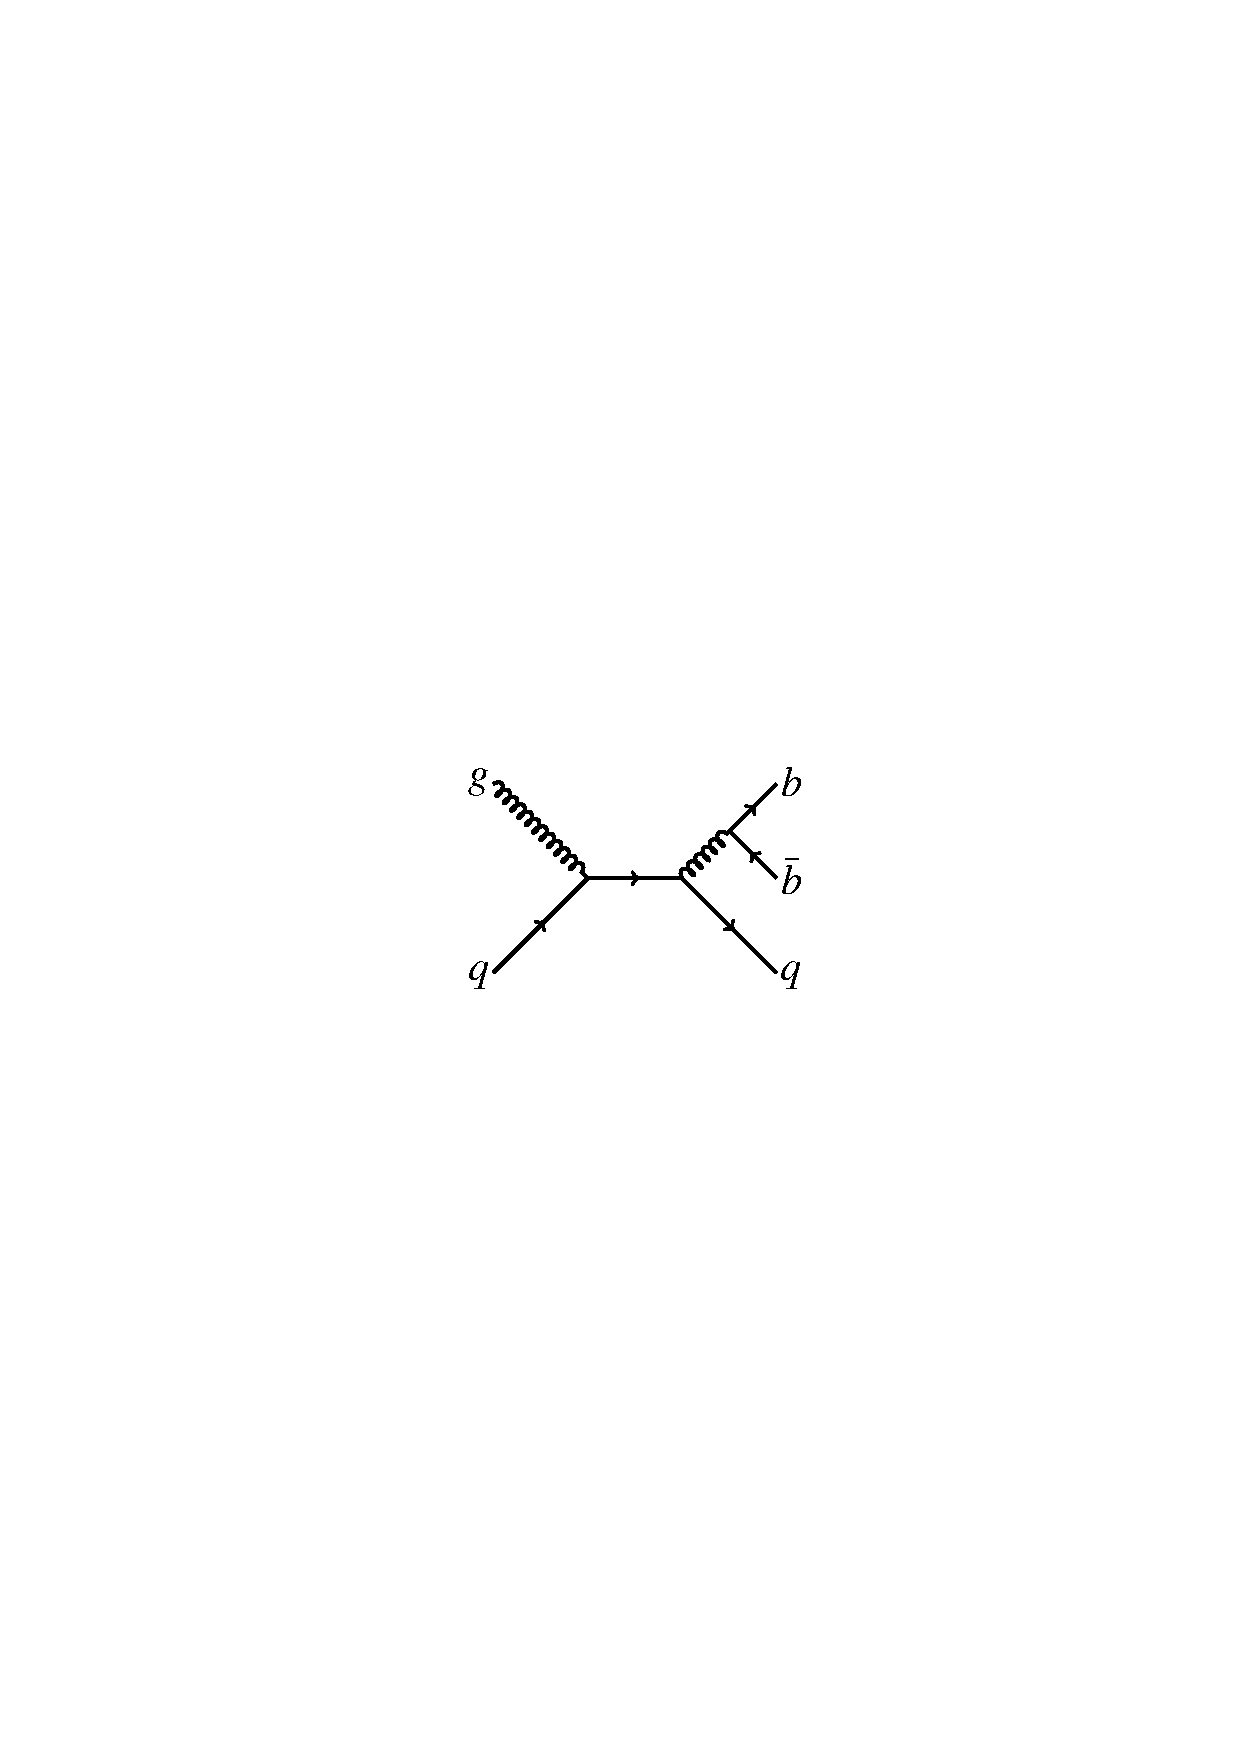
\includegraphics[width=0.5\textwidth]{figures/gbb/gbb_feynman}
\caption{Feynman diagram of gluon splitting to $b\bar{b}$}
  \label{fig:gbb-feynman}
\end{figure}


In this Chapter, we present a measurement of the differential properties of the gluon splitting vertex. The high transverse momentum and low angular separation regime for \gbb can be probed using large-radius jets with $b$-tagged small radius jets. A number of variables which characterize the \gbb vertex are defined in Sec.\ref{sec:gbb-var}. In the past, this topology has been used for calibrating $b$-tagging in dense environments~\cite{ATLAS-CONF-2016-039,ATLAS-CONF-2016-002,CMS:2013vea} and has been studied phenomenologically~\cite{Anderle:2017qwx,Ilten:2017rbd}. This measurement builds on these studies by first selecting events with one $R=1.0$ calorimeter jet and two $R=0.2$ track jets (Sec.\ref{sec:gbb-selection}) from the inclusive multi-jet sample. The flavor composition estimated by the simulated MC samples are usually not correct. Hence a flavor correction based on \sdzero template fit is performed before the background subtraction is made to data shown in Sec.\ref{sec:gbb-bkgsub} and Sec.\ref{sec:gbb-bkgres}. Reconstructed level background subtracted \gbb vertex variable distributions are then unfolded to truth jet level using iterative Bayes method\ref{sec:gbb-unfolding}. Comparisons between data and MC are shown in Sec.\ref{sec:gbb-results}.
